\documentclass[a4paper,12pt]{article}
\usepackage{a4wide}
\usepackage{tikz}
\usetikzlibrary{calc}

\begin{document}
\pagestyle{empty}
\setlength{\parindent}{0em} 
\section*{Truth Table}

Your task is to program the behavior of an entity called "truth\_table". This entity is declared in the attached file "truth\_table.vhdl" and has the following properties:
\begin{itemize}
\item Inputs:  A, B, C, D with type std\_logic
\item Outputs: O with type std\_logic
\end{itemize}

\begin{center}
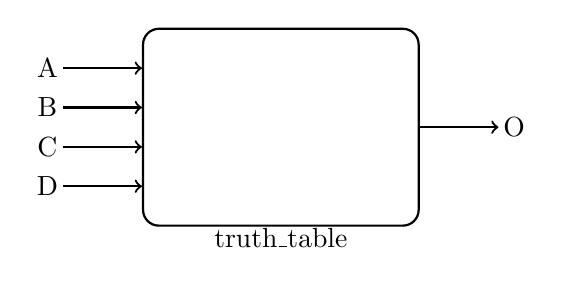
\begin{tikzpicture}
\draw node [draw,rectangle, minimum height=25mm, minimum width=35mm,rounded corners=2mm,thick](entity){};
\draw[->,thick] ($ (entity.west)-(10mm,7.5mm)$) -- ($ (entity.west) - (0mm,7.5mm)$);
\draw node at ($ (entity.west)-(12mm,7.5mm)$){D};
\draw[->,thick] ($ (entity.west)-(10mm,2.5mm)$) -- ($ (entity.west) - (0mm,2.5mm)$);
\draw node at ($ (entity.west)-(12mm,2.5mm)$){C};
\draw[->,thick] ($ (entity.west)-(10mm,-2.5mm)$) -- ($ (entity.west) - (0mm,-2.5mm)$);
\draw node at ($ (entity.west)-(12mm,-2.5mm)$){B};
\draw[->,thick] ($ (entity.west)-(10mm,-7.5mm)$) -- ($ (entity.west) - (0mm,-7.5mm)$);
\draw node at ($ (entity.west)-(12mm,-7.5mm)$){A};

\draw[->,thick] (entity.east) -- ($ (entity.east) + (10mm,0)$);;
\draw node at ($ (entity.east) + (12mm,0)$){O};

\draw node at ($ (entity) - (0,14mm)$){truth\_table};

\end{tikzpicture}
\end{center}

Do not change the file "truth\_table.vhdl".
\\

The "truth\_table" entity shall behave according to the following truth table:

\vspace{0.3cm}
\begin{center}
\begin{tabular}{||l | l | l | l || l||} 
	\hline
	D & C & B & A & O\\ [0.5ex] 
	\hline\hline
	0&0&0&0& %%O0
	\\
	\hline
	0&0&0&1& %%O1
	\\
	\hline
	0&0&1&0& %%O2
	\\
	\hline
	0&0&1&1& %%O3
	\\
	\hline\hline
	0&1&0&0& %%O4
    \\
	\hline
	0&1&0&1& %%O5
	\\
	\hline
	0&1&1&0& %%O6
	\\
	\hline
	0&1&1&1& %%O7
	\\
	\hline\hline
	1&0&0&0& %%O8
	\\
	\hline
	1&0&0&1& %%O9
	\\
	\hline
	1&0&1&0& %%O10
	\\
	\hline
	1&0&1&1& %%O11
	\\
	\hline\hline
	1&1&0&0& %%O12
	\\
	\hline
	1&1&0&1& %%O13
	\\
	\hline
	1&1&1&0& %%O14
	\\
	\hline
	1&1&1&1& %%O15
	\\
	\hline\hline
\end{tabular}
\end{center}

\vspace{0.3cm}

This behavior has to be programmed in the attached file "truth\_table\_beh.vhdl". Prior simplification with an
optimization algorithm like Karnaugh Veith (KV diagram) is encouraged.
\\

To turn in your solution write an email to %%SUBMISSIONEMAIL with Subject "Result Task %%TASKNR" and attach your file "truth\_table\_beh.vhdl".

\vspace{0.7cm}
Good Luck and May the Force be with you.


\end{document}
